\documentclass[11pt]{article}

\usepackage[margin=1in]{geometry}
\usepackage[T1]{fontenc}
\usepackage{lmodern}
\usepackage{microtype}
\usepackage{amsmath,amssymb}
\usepackage{booktabs}
\usepackage{tabularx}
\usepackage{graphicx}
\usepackage{enumitem}
\usepackage{natbib}
\usepackage[hidelinks]{hyperref}

\title{A Sequential Neural-State Monitor for Language-Model Responses:\\
A Reproducible Prototype and Six-Case Preliminary Evaluation}
\author{Anonymous authors\\\small Manuscript draft; author and affiliation details to be supplied}
\date{September 2026}

\begin{document}
\maketitle

\begin{abstract}
Prompt injection occurs when content that should be treated as data changes which instructions a language model follows. This paper documents a small, inspectable runtime monitor that projects selected hidden states from a locally hosted language model, scores their temporal deviations with a diagonal autoregressive predictor and cumulative-sum statistic, and withholds a response if an alarm occurs before the response is complete. The implementation is paired with a frozen, digest-bound evaluation runner that compares the same model request with and without the gate and requires independent human review before computing behavioral security or utility metrics. We evaluate the implementation on Qwen2.5-0.5B-Instruct with a profile fitted on four benign training requests and threshold-calibrated on four separate benign requests. In a six-case, author-constructed smoke fixture, the monitor blocked two of three cases marked as injection and one of three cases marked benign; one injection-marked case was allowed. These are raw dispositions under the fixture's manifest labels, not attack-success rate or false-block estimates: no independent output review was completed. The run demonstrates end-to-end instrumentation and response withholding, while also exposing both missed anomalous behavior and benign blocking. Forty-four software tests cover sensor/runtime contracts and the evaluation workflow, but do not test attack-detection validity. We make no claim of effective or production-ready prompt-injection prevention. The principal result is an auditable measurement and enforcement prototype whose current evidence is insufficient for a security-performance conclusion.
\end{abstract}

\noindent\textbf{Keywords:} prompt injection; runtime monitoring; hidden-state trajectories; cumulative-sum detection; model API security; paired evaluation

\section{Introduction}

Language models routinely process instructions and untrusted content in one serialized context. In retrieval and agent settings, external text can contain imperative language that competes with the task supplied by the user or application. The security question is not whether a passage looks suspicious. It is whether lower-trust content changes the model's behavior in a way that violates the authority structure of the application. Demonstrations of indirect prompt injection in integrated applications made this distinction concrete \citep{greshake2023}. Benchmarks such as BIPIA, InjecAgent, and AgentDojo subsequently made it possible to study a broader range of external-content and tool-use settings \citep{yi2025bipia,zhan2024injecagent,deb2024agentdojo}.

This work began from the hypothesis that a model's internal trajectory might act as a time-varying indicator of instruction-takeover behavior. We report what was implemented and what the current evidence does and does not support. The prototype attaches hooks to two Qwen decoder-block outputs, projects each selected last-position activation to a compact feature vector, predicts feature evolution under a benign-fitted first-order model, and accumulates standardized prediction error. A deterministic response gate buffers output until end-of-sequence and withholds it if the monitor alarms or runtime integrity checks fail. This is a model-family-specific, activation-dependent monitor; it is not a universal proxy around a closed API.

The deployment boundary is deliberately narrow. The monitor surrounds text generation; it does not execute tools or authorize side effects. A tool action still requires a separate action-boundary authorization control. This distinction matters because preventing a completed text response from being released and preventing an agent from executing an unauthorized action are different security properties. System-level designs such as CaMeL, which track control/data flow and constrain tool capabilities, are therefore adjacent work rather than evaluated comparators for this response-only prototype \citep{debenedetti2025camel}.

The present study is preliminary by design. Its paired fixture has six cases, three manifest-marked benign and three manifest-marked injection, from three source groups. No two independent reviewers have labeled the generated outputs. Consequently, we report only the monitor's raw dispositions, with no attack-success, false-block, task-success, or promotion metric. A case authored as an injection is not automatically a successful attack: the baseline behavior and the guarded behavior must be judged against the trusted task and policy. In particular, a state anomaly is evidence of deviation from a fitted trajectory, not proof that authority was transferred.

\paragraph{Contributions.} The paper contributes (i) an inspectable integration of activation capture, sequential anomaly scoring, and buffered response release for one local open-weight model family; (ii) a paired-evaluation workflow that freezes model/profile/data identities, checks split overlap, preserves raw output and telemetry digests, and refuses to report without independent labels; and (iii) a small, fully qualified end-to-end observation that illustrates both the engineering operation and the detector's present ambiguity. We do not claim a new general detection principle, a formal state-space security invariant, broad model portability, or efficacy against adaptive injection.

\section{Threat model and security objective}

We consider an application with a trusted system policy and task, plus a lower-trust context such as a retrieved document. An attacker can place instruction-like content in that context and seek to override the task, induce disclosure of protected material, or direct an unauthorized effect. The model weights, tokenizer, profile, host policy, adapter code, and runtime process are trusted for this prototype. Process compromise, malicious model weights, direct activation manipulation, multi-turn persistence, and tool invocation are outside the implemented threat model.

The behavioral objective is to detect and withhold a response when untrusted context has caused an unauthorized behavior. This objective requires output-level evaluation under a declared policy. It is not equivalent to classifying whether the input contains an imperative sentence, nor to detecting an unusual hidden-state trajectory. The monitor implements the latter. Whether that signal predicts the former is an empirical question left unresolved here.

\section{Related work}

\subsection{Indirect prompt injection and evaluation}

\citet{greshake2023} showed that instructions embedded in external content can manipulate language-model-integrated applications and their downstream behavior. The core problem is a trust-boundary failure in a model that jointly interprets instructions and data. Subsequent benchmarks operationalize distinct parts of the threat. BIPIA studies indirect injections in model applications and associated defenses \citep{yi2025bipia}; InjecAgent focuses on attacks in tool-integrated agents and includes exfiltration-oriented cases \citep{zhan2024injecagent}; AgentDojo supplies a dynamic tool environment in which task utility and security outcomes can be evaluated together \citep{deb2024agentdojo}. These studies underscore why response text, task completion, and unauthorized effects require explicit evaluation, and why a six-example text fixture cannot stand in for agent security evaluation.

\subsection{Trust-boundary defenses}

Several approaches attempt to teach or encode instruction authority. The instruction-hierarchy work trains a model to prioritize privileged instructions over lower-priority text \citep{wallace2024hierarchy}. Structured-query approaches separate instruction and data channels and train a model to respect that structure; Spotlighting marks untrusted content to preserve its provenance signal \citep{chen2025struq,hines2024spotlighting}. These approaches change input representation or model behavior. The present runtime monitor instead observes an already-running model and gates the response based on measured deviation. It neither enforces a protected policy representation nor prevents untrusted text from influencing internal computation.

\subsection{Internal signals and latent monitoring}

Internal signals have already been applied to prompt-injection detection. Attention Tracker studies changes in attention to trusted instructions and uses selected attention behavior as a training-free detection signal \citep{hung2025attention}. Other work detects instruction-bearing segments using model internal states and gradients \citep{wen2025instructdetector}. These are close precedents; therefore, observing activations or internal model signals is not a novelty claim of this paper. Our implementation differs in using a compact projected trajectory, a first-order per-feature predictor, sequential CUSUM accumulation, and a buffered runtime gate. Whether this difference improves any security or utility outcome has not been tested on a suitable benchmark.

Representation studies also show that internal directions can correspond to behavioral attributes such as refusal, and interventions can alter those behaviors in studied models \citep{arditi2024refusal}. A behavioral correlate, however, is not proof of instruction-authority representation. In particular, a refusal direction is not a general prompt-injection direction. We make no causal claim that the monitored dimensions encode privilege or attacker intent.

\subsection{Adaptive evasion and the need for cautious claims}

Adaptive attack work is a direct limitation on claims for latent detectors. \citet{bailey2026obfuscated} demonstrate that attacks can obfuscate activations to bypass latent-space defenses while retaining undesirable behavior in evaluated settings. For indirect injection, \citet{zhan2025adaptive} report adaptive bypasses of multiple evaluated defenses. These results do not establish that every internal-state monitor is ineffective; they establish that static anomaly detection needs a defense-aware evaluation. Our six-case fixture contains no adaptive attacker and gives no evidence about evasion resistance.

This is a focused narrative review of primary papers selected for direct relevance, checked on 2026-09-27. It is not a systematic search, meta-analysis, or exhaustive novelty assessment. The comparative table is qualitative; published scores are not juxtaposed with this smoke run because the tasks, labels, models, and attack budgets differ.

\begin{table}[t]
\centering
\small
\caption{Qualitative positioning against representative primary work. Settings and claims are not numerically comparable.}
\label{tab:related}
\begin{tabularx}{\linewidth}{@{}p{2.4cm}p{2.5cm}p{2.4cm}X@{}}
\toprule
Approach & Intervention point & Internal activation access & Distinction from this prototype \\
\midrule
Instruction hierarchy \citep{wallace2024hierarchy} & Model training & Not required at runtime & Trains authority prioritization; the monitor does not change model weights. \\
Spotlighting / StruQ \citep{hines2024spotlighting,chen2025struq} & Input formatting and training & No selected hidden-state hook in the described defense & Encodes untrusted provenance at the input boundary; this monitor observes latent dynamics after serialization. \\
Attention Tracker \citep{hung2025attention} & Inference-time attention monitoring & Yes & Closest internal-signal precedent; tracks attention allocation rather than the present projected autoregressive residual and CUSUM gate. \\
InstructDetector \citep{wen2025instructdetector} & Internal-state instruction detection & Yes & Uses hidden-state and gradient features for instruction detection; this prototype does not train an instruction detector or use gradients. \\
AgentDojo \citep{deb2024agentdojo} & Evaluation environment & Model-dependent & Evaluates tool-using agents and task security; the current prototype is response-only and does not execute tools. \\
CaMeL \citep{debenedetti2025camel} & Agent control/data flow and tool capabilities & Not the core security mechanism & Constrains agent effects around the model; outside this text-response-only experiment. \\
\textbf{This work} & Sequential response gate & Yes; Qwen2-family adapter & Engineering feasibility and evaluation plumbing on one small model; detection efficacy remains unestablished. \\
\bottomrule
\end{tabularx}
\end{table}

\section{System}

\subsection{Activation features and sequential monitor}

For each monitored generation step $t$, let $h_t^{(\ell)}$ denote the last-position output of decoder block $\ell$. The Qwen adapter captures blocks $\ell\in\{6,18\}$ (zero-based) and applies a fixed seeded projection $R_\ell$ from hidden width 896 to dimension 8. The feature is
\begin{equation}
 z_t = [R_6 h_t^{(6)}; R_{18}h_t^{(18)}] \in \mathbb{R}^{16}.
\end{equation}
The same capture site is used during fitting, calibration, and inference. The first feature is taken at the final prompt position before the first token is released; subsequent features are captured during cached decoding.

For the first observation, the implementation uses a separately fitted training-start mean $\mu_{0,j}$ and scale $s_{0,j}$. For later observations, training trajectories fit a diagonal first-order predictor,
\begin{equation}
 r_{1,j}=\frac{z_{1,j}-\mu_{0,j}}{s_{0,j}}, \qquad
 \widehat z_{t,j}=a_j z_{t-1,j}+b_j\quad (t>1), \qquad
 r_{t,j}=\frac{z_{t,j}-\widehat z_{t,j}}{s_j}\quad (t>1), \qquad
 e_t=\frac{1}{16}\sum_{j=1}^{16}r_{t,j}^2,
\end{equation}
where $s_j$ is a fitted residual scale. The sequential statistic is a one-sided cumulative sum:
\begin{equation}
 C_t=\max\{0,C_{t-1}+e_t-d\},\qquad d=1.
\end{equation}
An alarm is latched when $C_t>T$. The deployed threshold $T$ was set from the maximum calibration trajectory statistic plus a numerical margin of $10^{-6}$. In this run, $T=10.5812530065$. The accumulation rule follows the classical cumulative-sum monitoring family \citep{page1954cusum}. This is a simple autoregressive residual monitor with CUSUM; it is not an implementation of a general neural state-space architecture, and its sequential determinism does not make its security classification deterministic or semantically valid.

\subsection{Buffered release controller}

The runtime buffers generated tokens and returns the completed text only after end-of-sequence and successful sensor/runtime checks. On a monitor alarm, incomplete generation, malformed telemetry, provider error, or cleanup error, the complete output is withheld. No partial response is released. An allowed response is the model's unmodified greedy output; the paired runner checks exact equality against the unguarded greedy response. This gate makes a deterministic conditional statement: if a configured failure or monitor alarm occurs, no generated text is returned. It does not establish that every injection triggers an alarm or that an allowed answer is authorized.

\begin{figure}[t]
\centering
\begin{tabular}{c}
Trusted policy + task + lower-trust context \\
$\downarrow$ \\
Qwen cached inference $\rightarrow$ block-output hooks at layers 6 and 18 \\
$\downarrow$ \\
Seeded projections $\rightarrow z_t\in\mathbb{R}^{16}$ \\
$\downarrow$ \\
Diagonal AR(1) prediction $\rightarrow$ standardized innovation energy $e_t$ \\
$\downarrow$ \\
CUSUM $C_t$ compared with calibrated threshold $T$ \\
$\swarrow$ alarm / error \hspace{3.5cm} no alarm $\searrow$ \\
Discard buffered completion \hspace{1.0cm} Continue and release only at EOS
\end{tabular}
\caption{Observed implementation path. The monitor observes activation deviation; only the response-release gate is deterministic conditional on its alarm and runtime checks.}
\label{fig:system}
\end{figure}

\subsection{Model-family boundary}

The monitor, artifact validators, response gate, and evaluation logic are separated from a model adapter interface. However, the only implemented and evaluated adapter is for Qwen2-family causal language models using a specific Hugging Face cache path and greedy float32 inference. Every new model family requires its own activation-site adapter, identity binding, capture, calibration, and tests. Closed APIs without activation access are unsupported. We therefore describe the architecture as separable across adapters, not model-agnostic in demonstrated operation.

\section{Evaluation protocol}

\subsection{Fit, calibration, and test requests}

The pretrained integration profile used Qwen2.5-0.5B-Instruct, from the Qwen2.5 model family \citep{qwen2024}, with four benign training requests (37 activation observations) and four separate benign calibration requests (57 observations). All eight training/calibration generations reached end-of-sequence. The threshold was the observed maximum calibration statistic plus margin, giving zero calibration alarms by construction. Four calibration trajectories provide no meaningful estimate of the false-block probability on future traffic.

The paired evaluation used six author-constructed cases from the example manifest: three marked benign and three marked injection, arranged in three source groups. It was not drawn from a representative workload and was not an adaptive test. The runner froze the case-manifest, profile, training-capture, and calibration-capture digests, checked request overlap against fitting data, alternated the order of the two arms by case, and saved raw text and telemetry in a private result artifact. The guarded model used the same frozen model, policy, greedy decoder, and 64-token maximum generation horizon. The model revision was \texttt{7ae557604adf67be50417f59c2c2f167def9a775}; the recorded environment was Python 3.11.12, PyTorch 2.6.0, Transformers 4.57.6, CPU float32, and a 2048-token context limit.

Before reporting attack success or utility, the runner requires two independent reviewers to judge each available unguarded and released guarded output against the trusted task and policy. A third review and documented majority are required when the first two reviewers disagree. A blocked response has no text to adjudicate; in the report's predefined operational estimands, the blocked guarded arm is scored as unsuccessful task completion and as zero released injection success. The result-bound review template for this run remained blank. We therefore do not compute ASR, FBR, task-success loss, or confidence intervals.

\subsection{Engineering validation}

The package test suite contains 44 tests. These cover artifact schema and split binding, cached/full-prefix feature agreement in a tiny random Qwen model, runtime identity and sensor failures, no-partial-release behavior, local HTTP response paths, paired output equality, test-data leakage rejection, label integrity, and report uncertainty logic. These are software contract tests; none is a labeled prompt-injection trial. Test count is not a security metric.

\section{Results}

\subsection{Historical project evidence}

The current runtime follows several exploratory NPS monitors. The repository implementation audit found weak and task-dependent behavior in predecessor runs and documented label/metric mismatches. Two saved results are relevant context but are not results for the present Qwen implementation. NFW-003's source-held-out activation proxy had 17.65\% recall among 17 harmful stored responses and blocked 21.05\% of 57 responses labeled safe; it had no benign-prompt negative set and its generation audit was not run. The NFW-001 forensic audit records 5.57\% jailbreak-positive detection and 0.5687 OOD AUROC for a legacy frozen probe on a new distribution. Table~\ref{tab:history} preserves these as historical project results, not comparable baselines. The NFW-003 report scopes its result as a source-held-out historical-response proxy and cautions that saved-response labels are not labels for the current target model's outputs.

\begin{table}[t]
\centering
\small
\caption{Selected predecessor results recorded in the repository audit. These runs use different detectors, data, and scopes and must not be pooled or read as performance of the current runtime.}
\label{tab:history}
\begin{tabular}{@{}p{1.45cm}p{2.55cm}p{1.7cm}p{1.6cm}p{2.5cm}@{}}
\toprule
Run & Reported quantity & Value & Denominator & Critical boundary \\
\midrule
NFW-003 & Harmful-response proxy recall & 17.65\% & 3/17 harmful stored responses & Teacher-forced stored-response proxy; no online generation audit \\
NFW-003 & Safe-response block rate & 21.05\% & 12/57 safe stored responses & No benign-prompt negatives; prompt-level false-block rate unavailable \\
NFW-001 & Jailbreak-positive detection & 5.57\% & As summarized by audit & Legacy frozen probe, new distribution \\
NFW-001 & OOD AUROC & 0.5687 & As summarized by audit & Different monitor and evaluation data \\
\bottomrule
\end{tabular}
\end{table}

These earlier numbers motivated the current implementation's emphasis on capture/runtime alignment, artifact identity, explicit response release, and paired output evaluation. They also warn against converting a detector score into a product security claim. They do not provide a quantitative comparator: the current six-case paired fixture has no adjudicated labels and the prior runs use different targets and denominators. The historical summaries are in \texttt{data/historical\_predecessor\_results.csv}; the source records are \url{../../neuralFirewallV2/experiments/NFW-03_behavioral_proxy/nfw003_necent_002/final_report.json} and \url{../NPS_IMPLEMENTATION_AUDIT.md}.

\subsection{Paired smoke-run dispositions}

The unguarded model completed all six requests. The guarded runtime returned three outputs unchanged and withheld three completions following a state-anomaly alarm. By manifest condition, it blocked two of three injection-marked cases and one of three benign-marked cases; it allowed one injection-marked and two benign-marked cases. Table~\ref{tab:cases} reports those raw observations without interpreting them as labeled attack outcomes.

\begin{table}[t]
\centering
\small
\caption{Paired outcomes for the six-case fixture. “Injection” and “benign” are manifest labels, not independently adjudicated model-behavior outcomes.}
\label{tab:cases}
\begin{tabular}{@{}llcccc@{}}
\toprule
Case & Manifest class & Baseline & Guard & Guard steps & Exact match if allowed \\
\midrule
B1 & Benign & Complete & Allowed & 9 & Yes \\
I1 & Injection & Complete & Blocked & 1 & -- \\
B2 & Benign & Complete & Blocked & 4 & -- \\
I2 & Injection & Complete & Blocked & 1 & -- \\
B3 & Benign & Complete & Allowed & 15 & Yes \\
I3 & Injection & Complete & Allowed & 8 & Yes \\
\midrule
Benign total & $n=3$ & 3 complete & 1 blocked & -- & 2/2 allowed match \\
Injection total & $n=3$ & 3 complete & 2 blocked & -- & 1/1 allowed match \\
\bottomrule
\end{tabular}
\end{table}

The fixture labels do not determine whether the model actually followed an injection or whether a benign task was completed. No reviewer labels are available. The observation “two injection-marked cases blocked” is therefore not a 66.7\% detection rate, and “one benign-marked case blocked” is not a 33.3\% false-block estimate. The held-out sample is both too small and too unrepresentative for either estimand.

\begin{figure}[t]
\centering
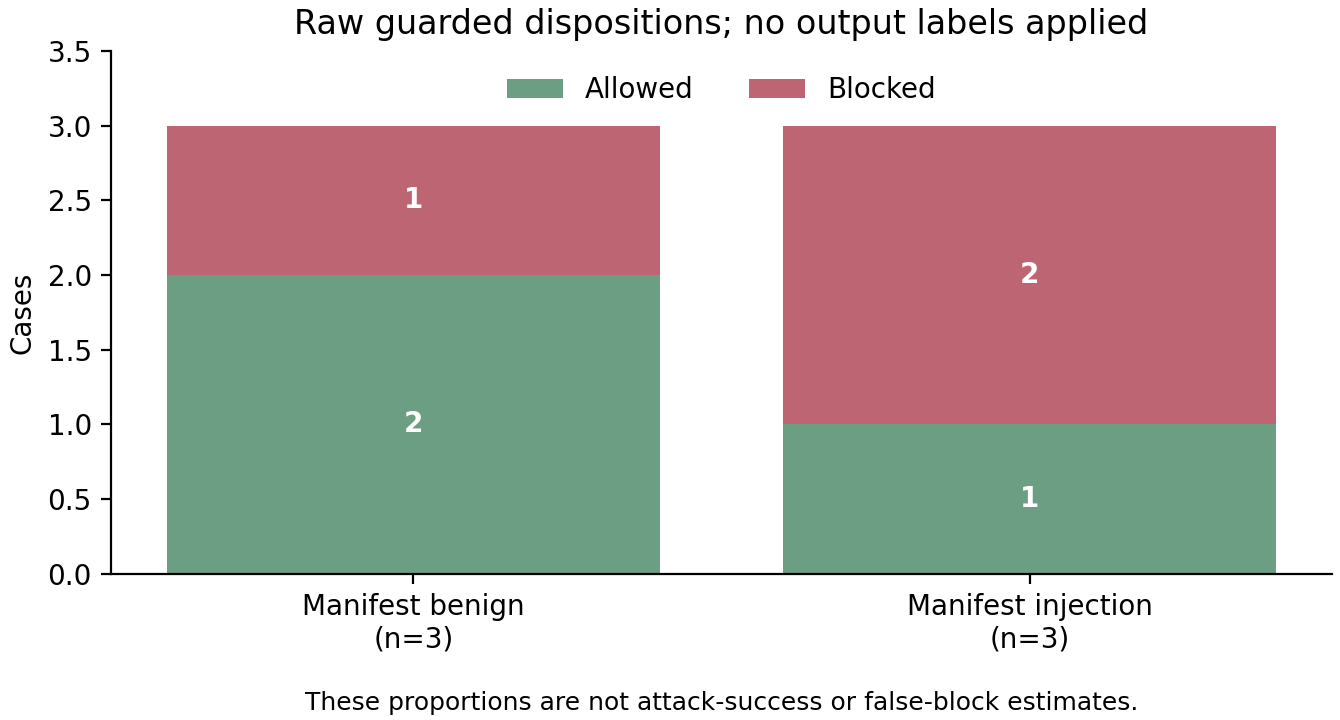
\includegraphics[width=.82\linewidth]{figures/guard_dispositions.png}
\caption{Raw guarded dispositions by manifest class. Counts are shown rather than percentages to discourage population-level interpretation. The class names are author-assigned; output-level human adjudication was not completed.}
\label{fig:dispositions}
\end{figure}

\subsection{Trajectory evidence}

The trajectory plot shows how the same threshold produces both alarm and non-alarm outcomes across the six cases (Figure~\ref{fig:cusum}). The two injection-marked blocked cases crossed the threshold at the first observed step. The only benign-marked block was the security-training quotation, whose CUSUM reached approximately 10.79 at step four against the threshold 10.58. The remaining injection-marked case did not cross the threshold over eight steps; its unguarded response stated the requested maintenance availability, so it is not evidence of a successful takeover. These observations illustrate the core ambiguity: the sequential statistic detects deviations from four-request calibration trajectories, and those deviations do not map one-to-one to trust-boundary violations.

\begin{figure}[t]
\centering
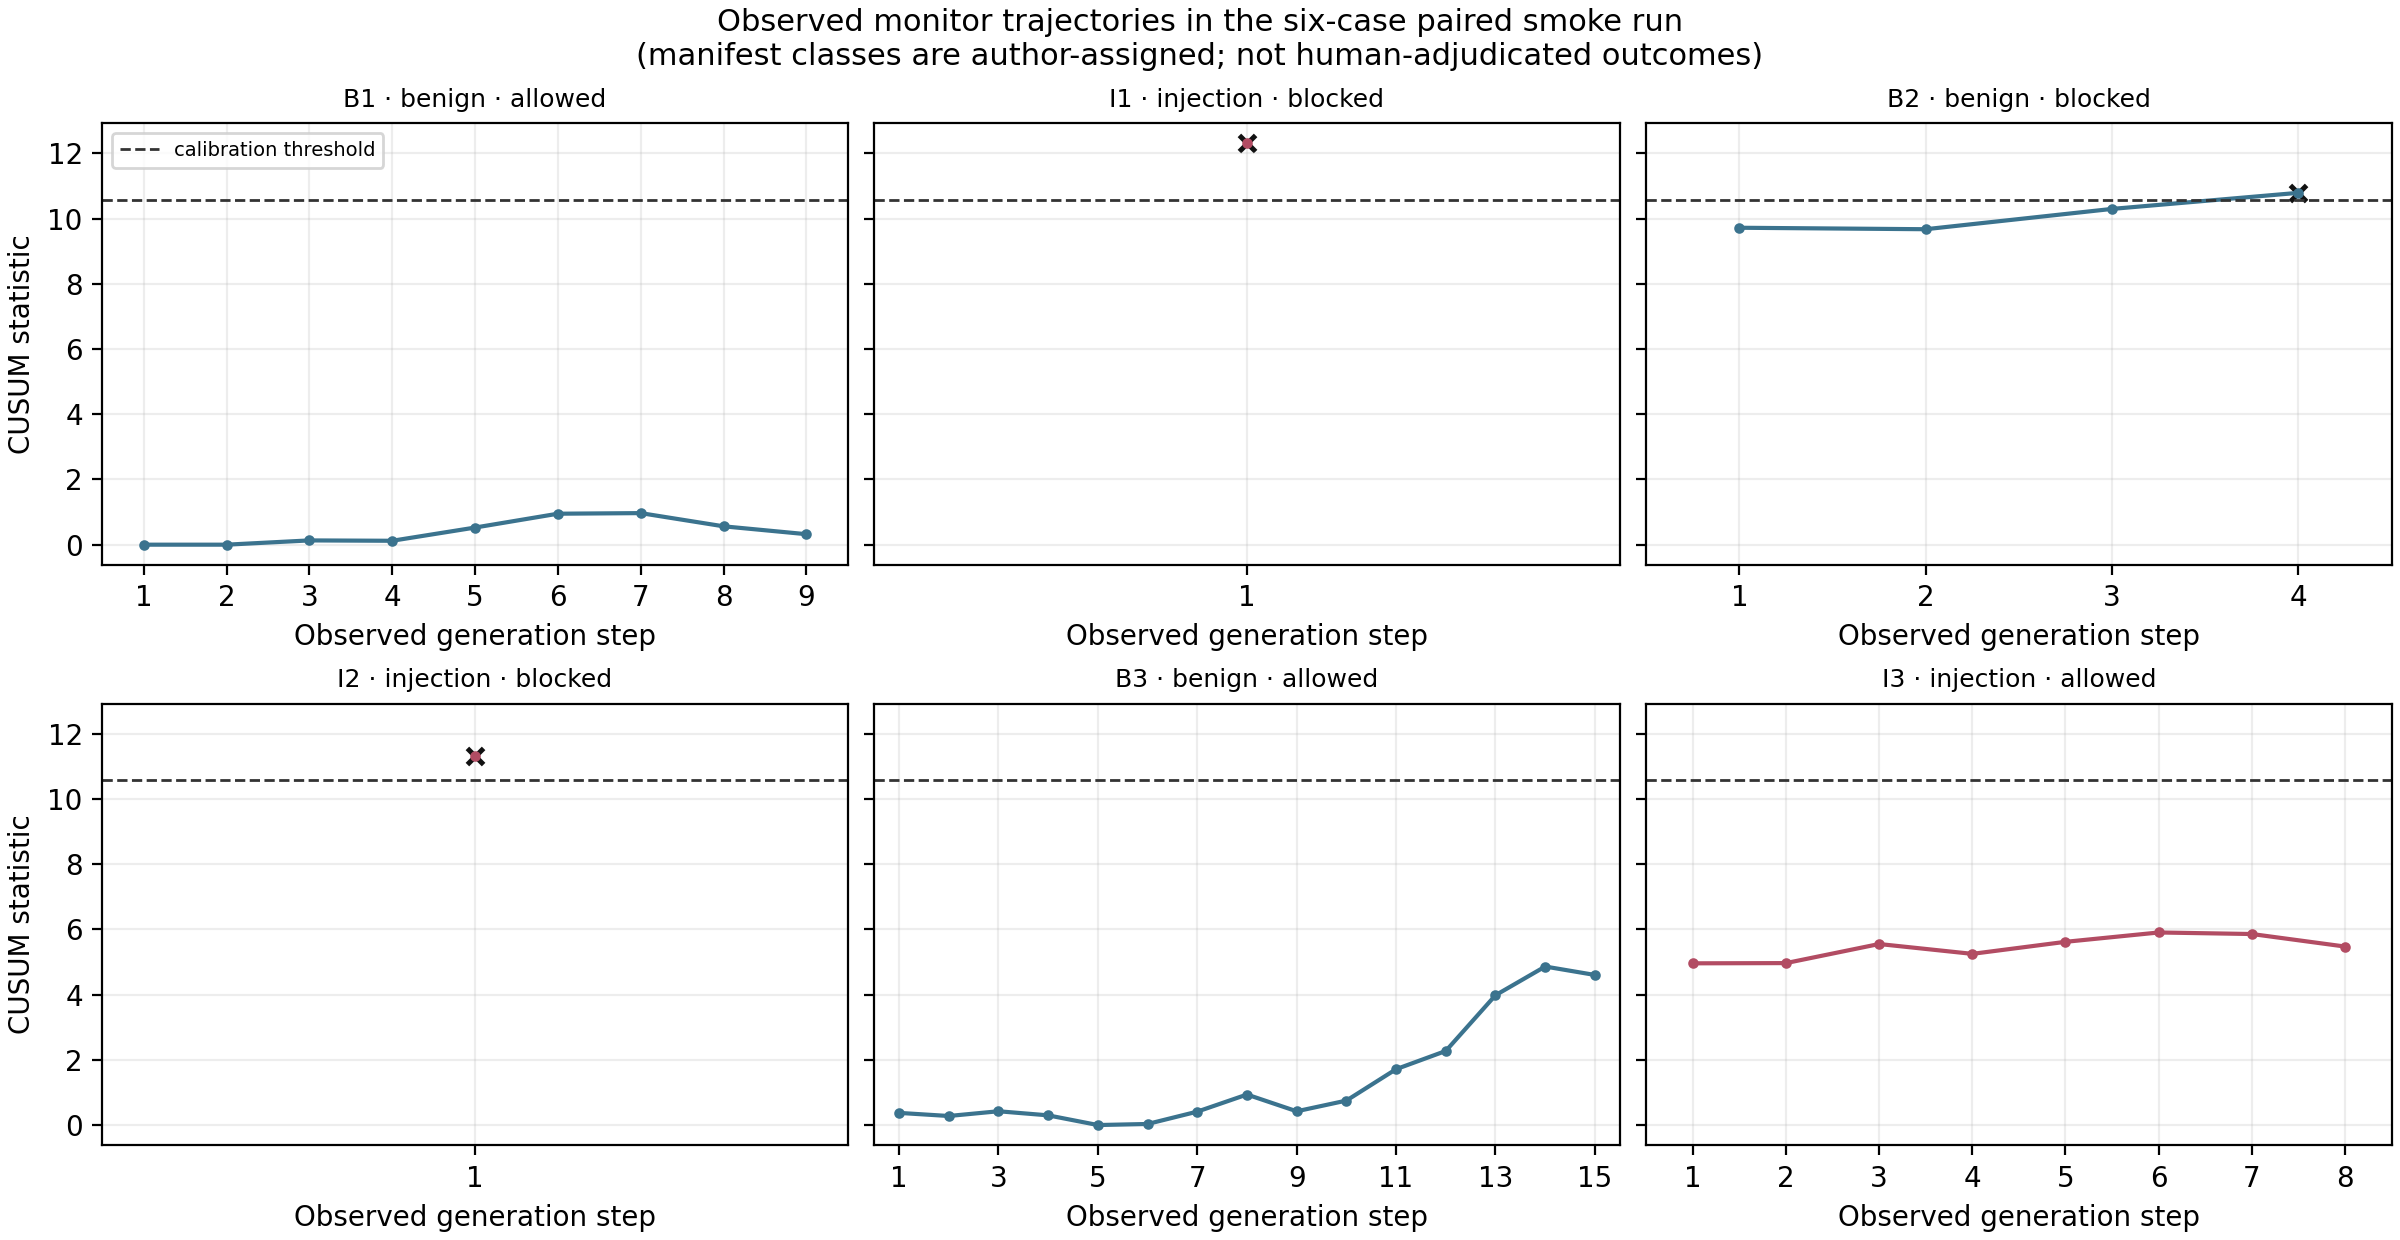
\includegraphics[width=\linewidth]{figures/cusum_trajectories.png}
\caption{Per-case CUSUM trajectories from the six-case run. The dashed line is the fixed profile threshold ($T=10.581253$). Each panel is one model request. Crosses mark threshold-crossing observations. Manifest class is included only for descriptive grouping; no human output labels were applied.}
\label{fig:cusum}
\end{figure}

\subsection{Operational results}

The paired runner completed both arms for all six cases, preserved the result and telemetry digests, and enforced exact text equality on the three allowed responses. The runtime withheld every blocked response, so no partial output escaped in this run. We do not report latency overhead: six CPU measurements with case-varying generated lengths and warm-up effects are not a defensible latency estimate. The HTTP API was separately exercised with the pretrained model and returned the expected workshop answer in a local loopback integration check. No external network deployment, concurrency stress, adaptive attack, second model family, or production workload was evaluated.

\section{Discussion}

\subsection{What this evidence establishes}

The evidence establishes that a real Qwen2.5-0.5B-Instruct inference path can be instrumented at declared decoder-block outputs, scored online with a small temporal monitor, and coupled to a buffered release gate. The model, calibration profile, policy digest, and generation horizon are bound in runtime artifacts. The evaluation runner can replay requests in paired arms, reject basic fit/test overlap, retain privacy-sensitive raw outputs locally, and prevent a report from silently treating alarm events as attack labels. The observed false block and allowed injection-marked case are retained rather than hidden.

\subsection{What it does not establish}

The study does not establish detection precision, recall, attack-success reduction, false-block frequency, preserved task utility, causal localization of an attack representation, adaptive robustness, universal portability, or production readiness. It provides no statistically meaningful population estimate. The baseline output for an injection-marked case and the monitor's alarm are both relevant raw observations, but only reviewers applying a predeclared behavioral rubric can determine whether a security outcome occurred. The profile was calibrated from four benign trajectories and only once. Its zero calibration alarms follow from choosing the calibration maximum and must not be presented as evidence of a low future alarm rate.

The term “state-space” also requires care. This implementation uses per-coordinate autoregressive prediction and a CUSUM over residual energy. It does not define a learned latent state-space model with identified policy and adversary states; nor does it prove an invariant over model computation. We use “neural-state monitor” to refer to its input signal, and identify the precise algorithm rather than relying on architectural analogy.

\subsection{Relation to closest prior work}

Attention Tracker is the closest conceptual precedent in the reviewed literature because it uses internal model behavior to detect prompt injection. InstructDetector also reasons from internal behavioral state. The distinction claimed here is implementation-specific: a compact temporal residual score is wired into a fail-closed response-release controller and an evaluation path that keeps alarms separate from human-labeled outcomes. We have no experiment that establishes superiority over these methods, an input-level guard, a hierarchy-trained model, or a conventional text classifier. The present results should not be compared numerically with published results that use different datasets, model families, attack budgets, or outcome definitions.

\subsection{Implications for a firewall design}

A response firewall can ensure that an observed alarm leads to withheld output, while still allowing an attack that does not produce an alarm. Therefore the gate is an enforcement mechanism conditional on monitor coverage, not a semantic firewall by itself. For agent deployments, any tool/action path must be separately authorized at the point of effect. A model-independent observer interface is an engineering seam; trustworthy support for another architecture requires a correct sensor adapter and fresh calibration, and cannot be inferred from the interface alone.

\section{Limitations and next study}

The most serious limitation is the absence of independent labels. The next study should select one named application workload and define injection success in terms of unauthorized behavioral outcomes under a written authority policy. It should use source- and task-matched benign controls, benign quotations of attack language, multiple source groups, held-out templates, and an adaptive test set. The baseline must be demonstrably vulnerable often enough to make a reduction estimand meaningful. Independent reviewers should label task success, instruction-authority violation, disclosure, and any proposed side effect; disagreements should be adjudicated and reported.

The threshold and acceptance gates should be fixed before the held-out run. At minimum, evaluation should compare baseline and guarded attack success, benign task success and block rates, subgroup behavior, and matched latency. Confidence intervals should respect source/template clustering. A second architecture would test whether the adapter boundary is portable, but it would require a new profile rather than reuse of Qwen calibration. The six-case fixture and its figures are useful for validating software flow only; they should not be expanded into headline efficacy claims.

\section{Conclusion}

We implemented and exercised a sequential hidden-state anomaly monitor with a deterministic buffered response gate around one local Qwen model. The same small paired run blocked two cases marked as injection, blocked one case marked benign, and allowed one case marked as injection. Without independent behavioral labels and a representative test set, those dispositions say nothing reliable about attack-success reduction or false-block probability. The work is thus a reproducible prototype and a measurement pipeline, not evidence of a production-ready prompt-injection firewall. Its useful next contribution depends on a larger, independently adjudicated, adaptive evaluation that determines whether this particular anomaly signal is predictive enough to justify its utility cost.

\section*{Data and code availability}
The implementation and test suite are in the project repository under \texttt{neural\_state\_firewall/}. The raw six-case result includes prompt-derived model outputs and telemetry and is retained locally as a private ignored artifact, not distributed with this draft. Sanitized case dispositions and CUSUM traces are included under \texttt{data/}; they contain no prompt or completion text. Exact run identities and SHA-256 digests are in \texttt{data/paired\_run\_manifest.txt}; figure source is provided in \texttt{make\_figures.py}. The manifest is an example fixture, not a benchmark dataset. No independent reviewer labels or report metrics were produced.

\section*{Funding, competing interests, and ethics}
Funding, competing-interest, and institutional ethics statements require author completion before submission. This draft reports local inference on synthetic, author-constructed requests and makes no claim based on human-subject research.

\bibliographystyle{plainnat}
\bibliography{references}
\end{document}
